%   +-------------+
%   |   RESULTS   |
%   +-------------+
\section{Results}\label{sec:result}

%   < Scheduling performance >
\subsection{Scheduling performance}\label{sec:res-sched}

\begin{figure}[p!]
    \centering
    \null\hfill
    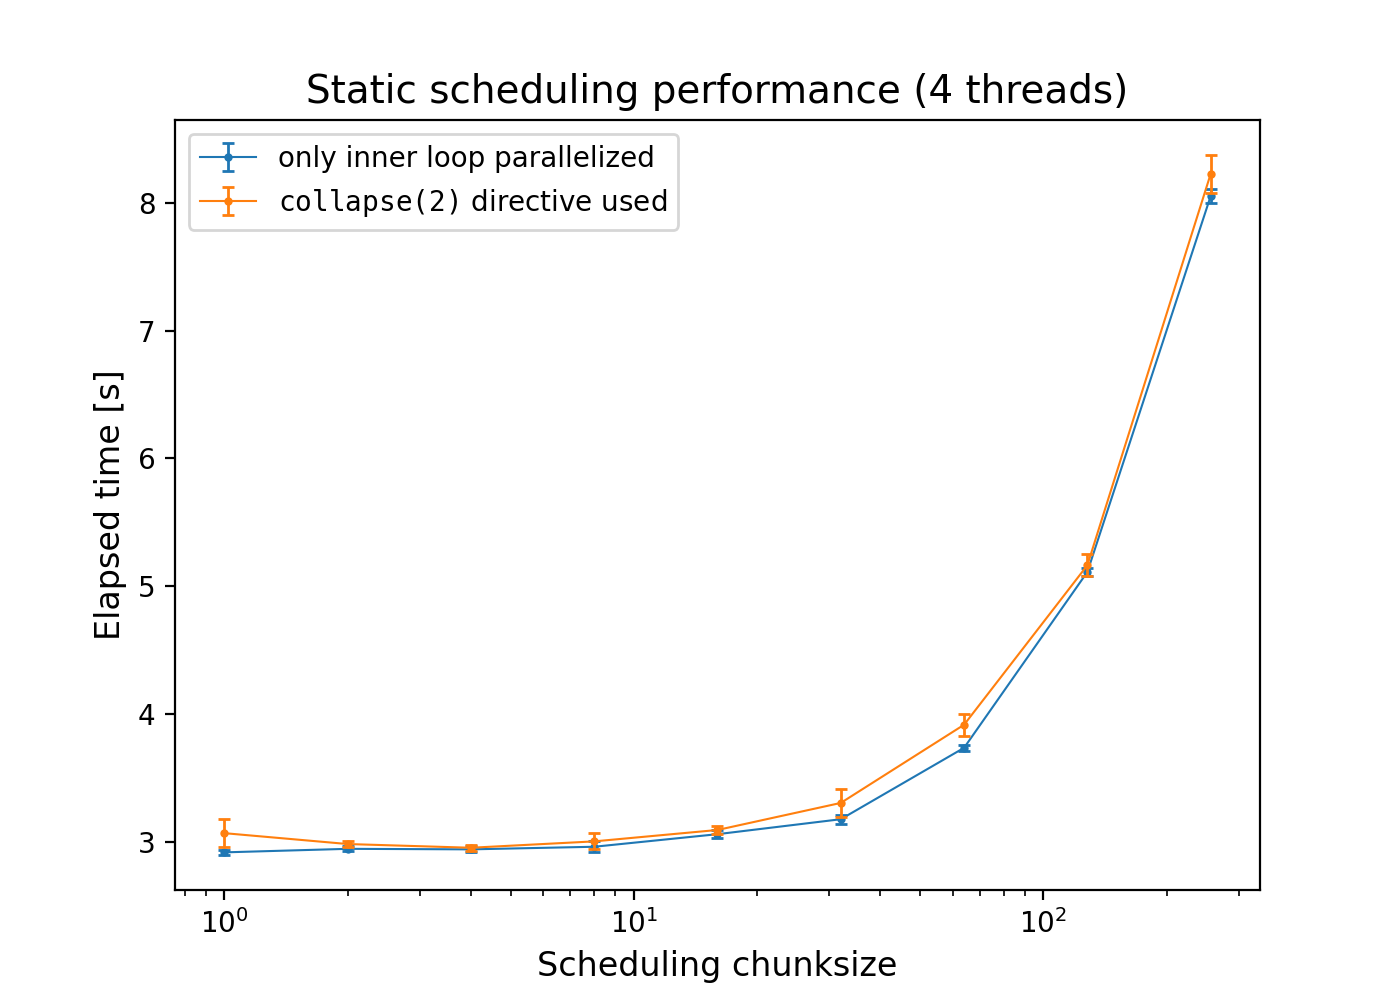
\includegraphics[width=0.49\textwidth]{sizeVStime_4threads_static.png}
    \null\hfill
    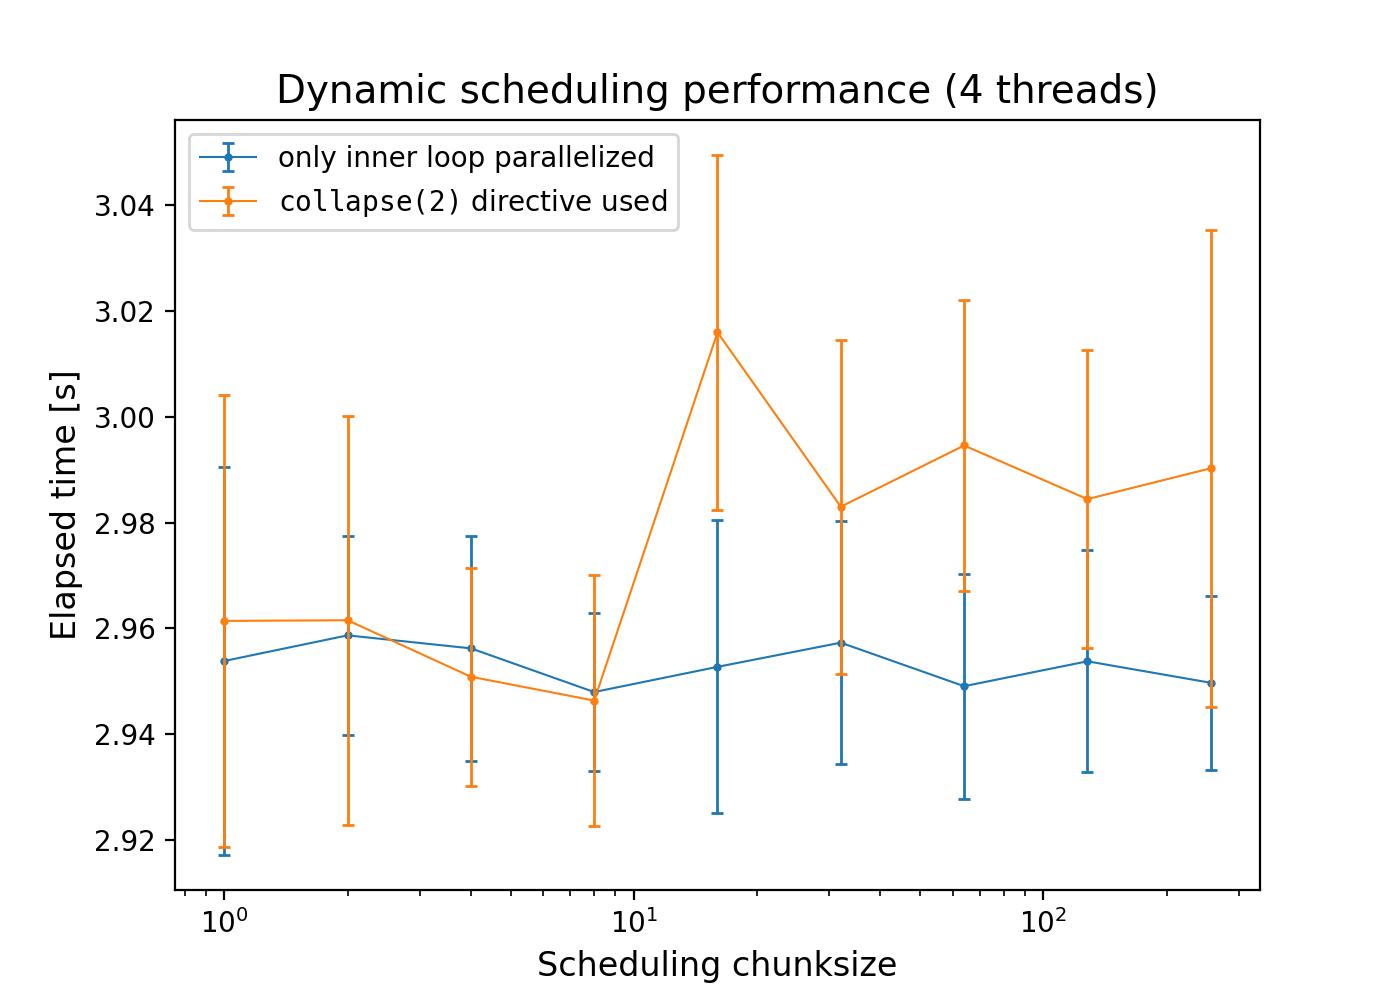
\includegraphics[width=0.49\textwidth]{sizeVStime_4threads_dynamic.png}
    \null\hfill
    \\
    \null\hfill
    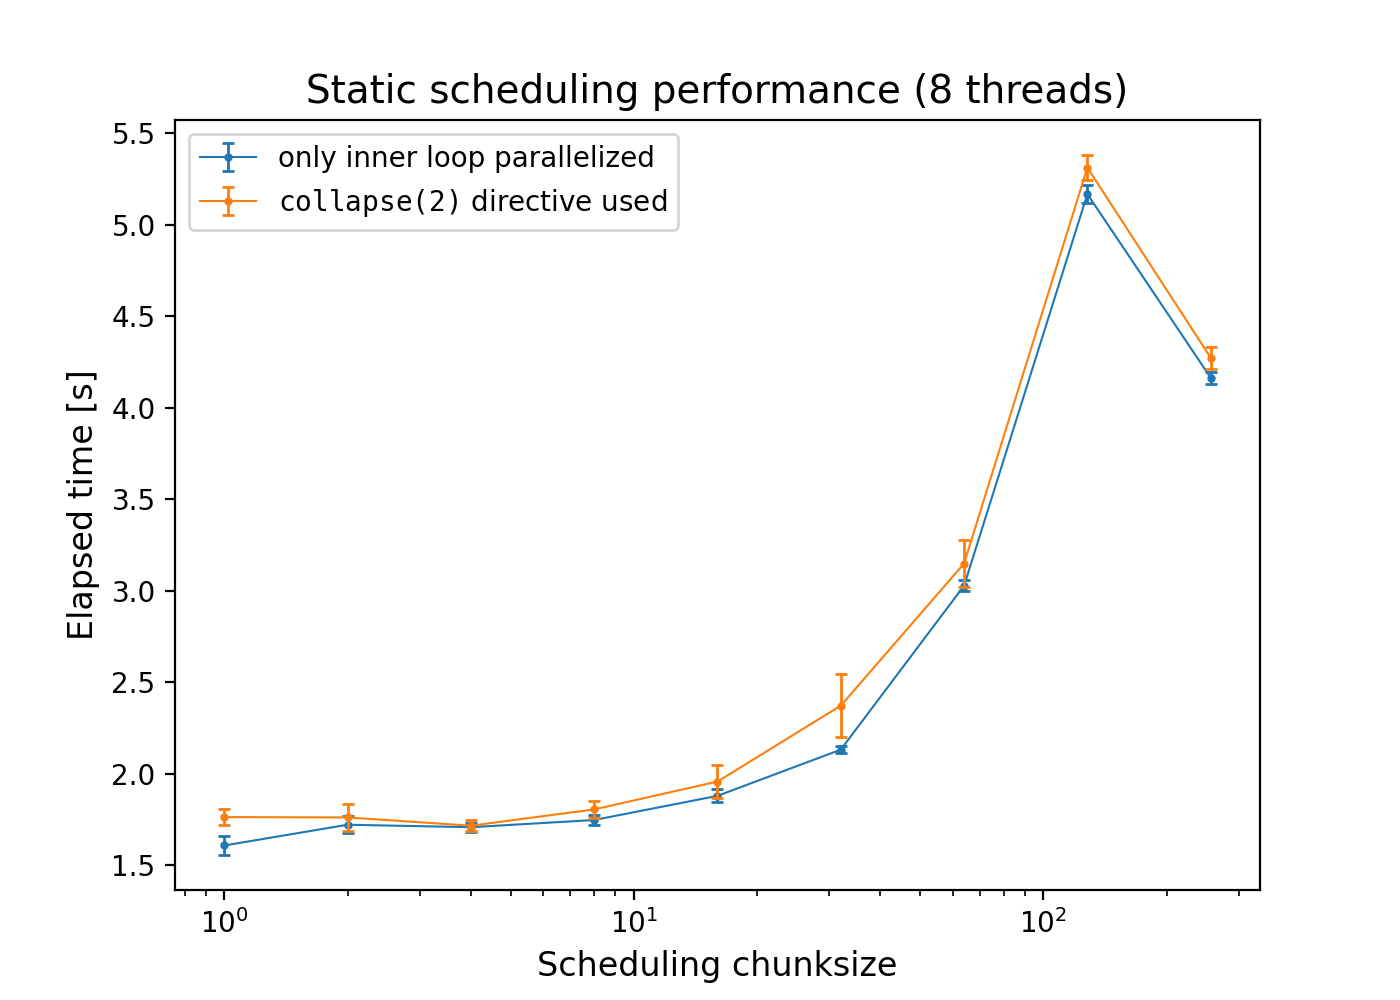
\includegraphics[width=0.49\textwidth]{sizeVStime_8threads_static.png}
    \null\hfill
    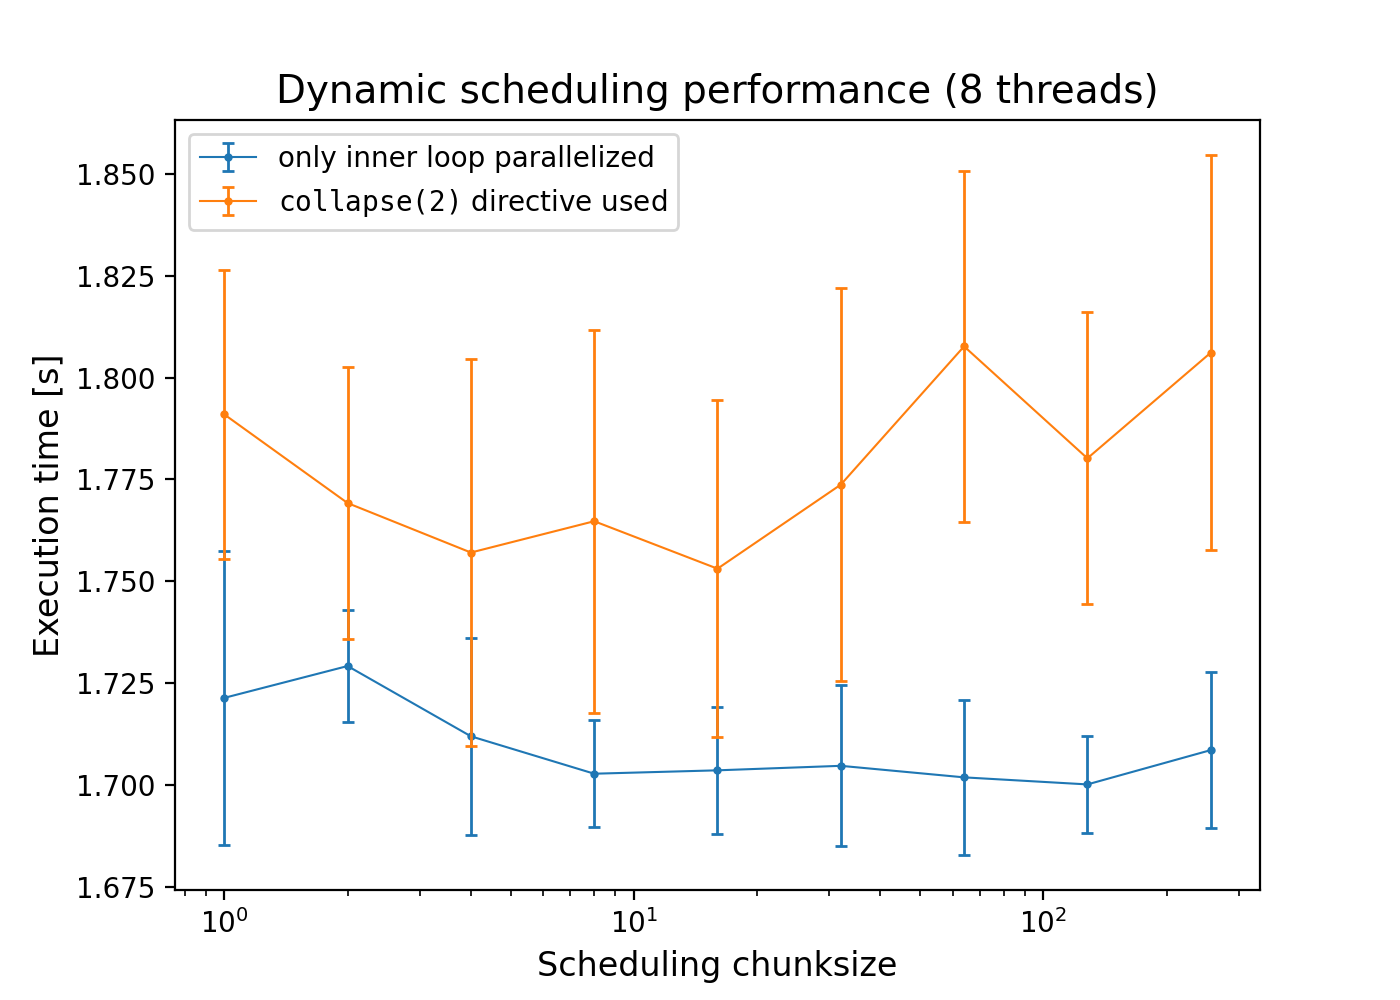
\includegraphics[width=0.49\textwidth]{sizeVStime_8threads_dynamic.png}
    \null\hfill
    \\
    \null\hfill
    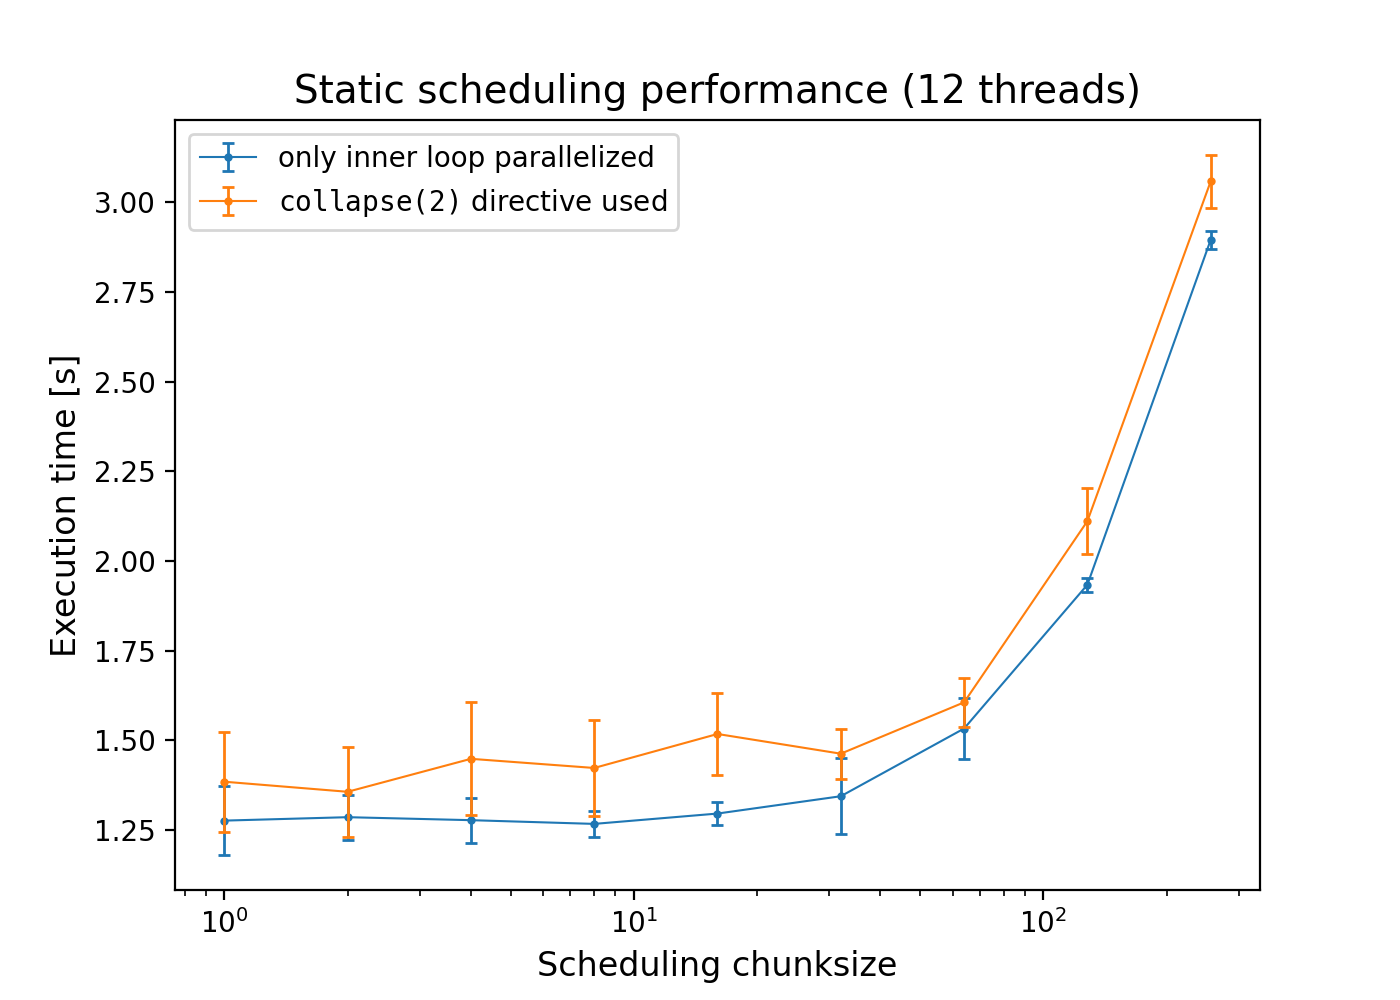
\includegraphics[width=0.49\textwidth]{sizeVStime_12threads_static.png}
    \null\hfill
    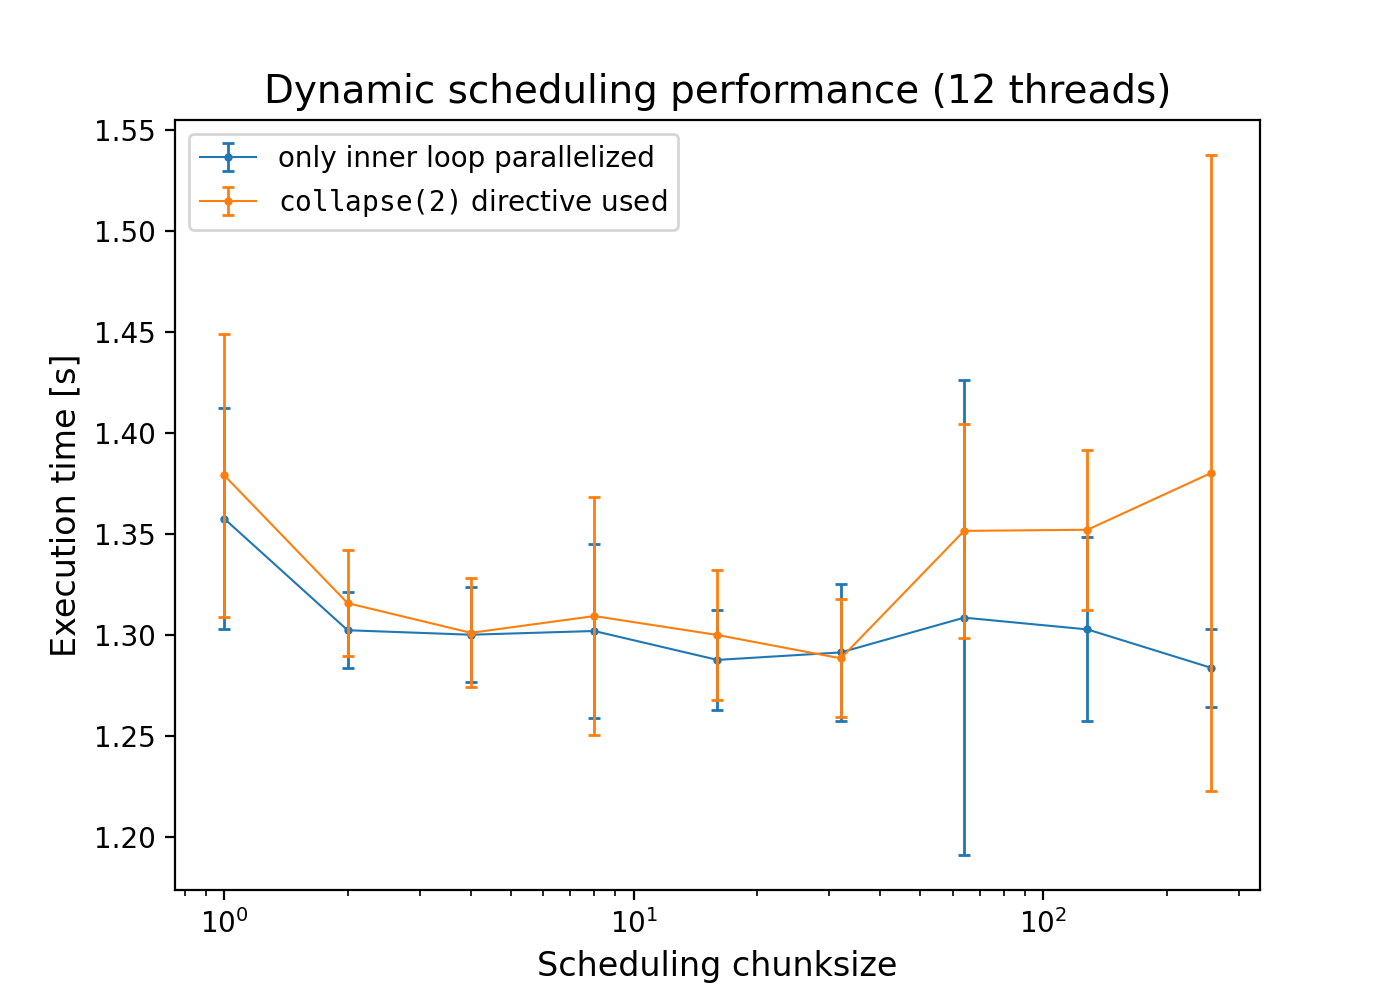
\includegraphics[width=0.49\textwidth]{sizeVStime_12threads_dynamic.png}
    \null\hfill
    \caption{\label{fig:sched}
    Performance curves of programs parallelized to compute the Mandelbrot set using 4, 8 and 12 threads. The left column reports the effect of enabling the \code{static} scheduling with different values of the chunksize in the elapsed times of a program with only the inner loop sped up (blue curves) and a program with the whole nested loop parallelized (orange curves). On the right column the same curves are reported using the \code{dynamic} scheduling.}
\end{figure}

The Figure~\ref{fig:sched} shows the time needed to compute the Mandelbrot set with respect to the partition size in \code{static} (left plots) and \code{dynamic} (right plots) scheduling conditions. Looking at the plots reported on the left column is clear that greater values of the scheduling chunksize leads to an increasing of the overhead. This is an expected behavior if we look at the graphical representation of the Mandelbrot set reported in Figure~\ref{fig:mandelbrot}: since the points with the highest computational cost are adjacent (the light brown ones), taking a large value for the chunksize corresponds to a high probability of assigning blocks of expensive computations to single threads, instead of distributing the workload as it happens with low values of the chunksize. On the contrary, the \code{dynamic} scheduling seems to be not affected by this drawback: a possible explanation is that the dynamic assignment of the workload allows to the quicker threads to handle the works more expensive, partially absorbing the overhead reported in \code{static} scheduling. However, I believe this isn't enough to describe what shown in the plots on the right column.

Another interesting results to derive from the plots in Figure~\ref{fig:sched} is a comparison in performance terms of the program with only the inner loop parallelized against the one that parallelizes the whole nested loop. Even if in most of the points the elapsed times seem to be consistent, the \code{collapse}-based program shows performance slightly worse than its counterpart. Again, we are looking at a non-completely understood behavior that maybe can be described like a sort of edge-phenomenon: in fact, the \ompcode{collapse(2)} clause allows to unroll the nested loop, leading the last iterations of the outer loop to be adjacent to the first ones of the next inner loop. Since the region near the edges almost doesn't require any computation (see the colors of the Figure~\ref{fig:mandelbrot}), it can lead to a greater probability of having the \emph{same} processors performing the heaviest work, for both \code{static} and \code{dynamic} scheduling. 

%   < Weak and strong scaling performance >
\subsection{Weak and strong scaling performance}\label{sec:res-scale}

\begin{figure}[b!]
    \centering
    \null\hfill
    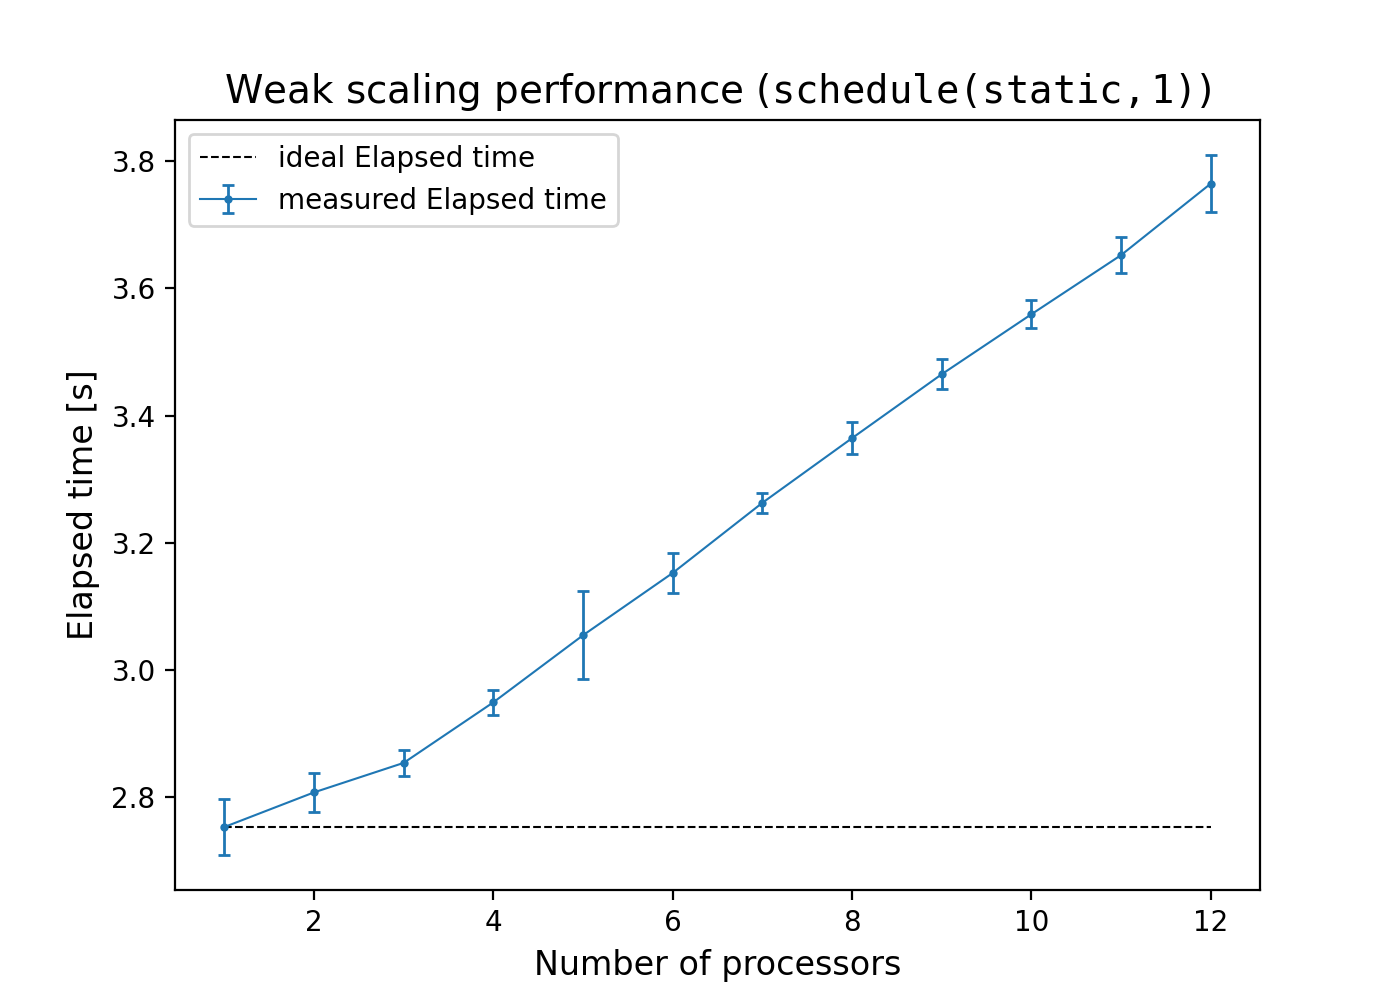
\includegraphics[width=0.42\textwidth]{threadsVStime_weak.png}
    \null\hfill
    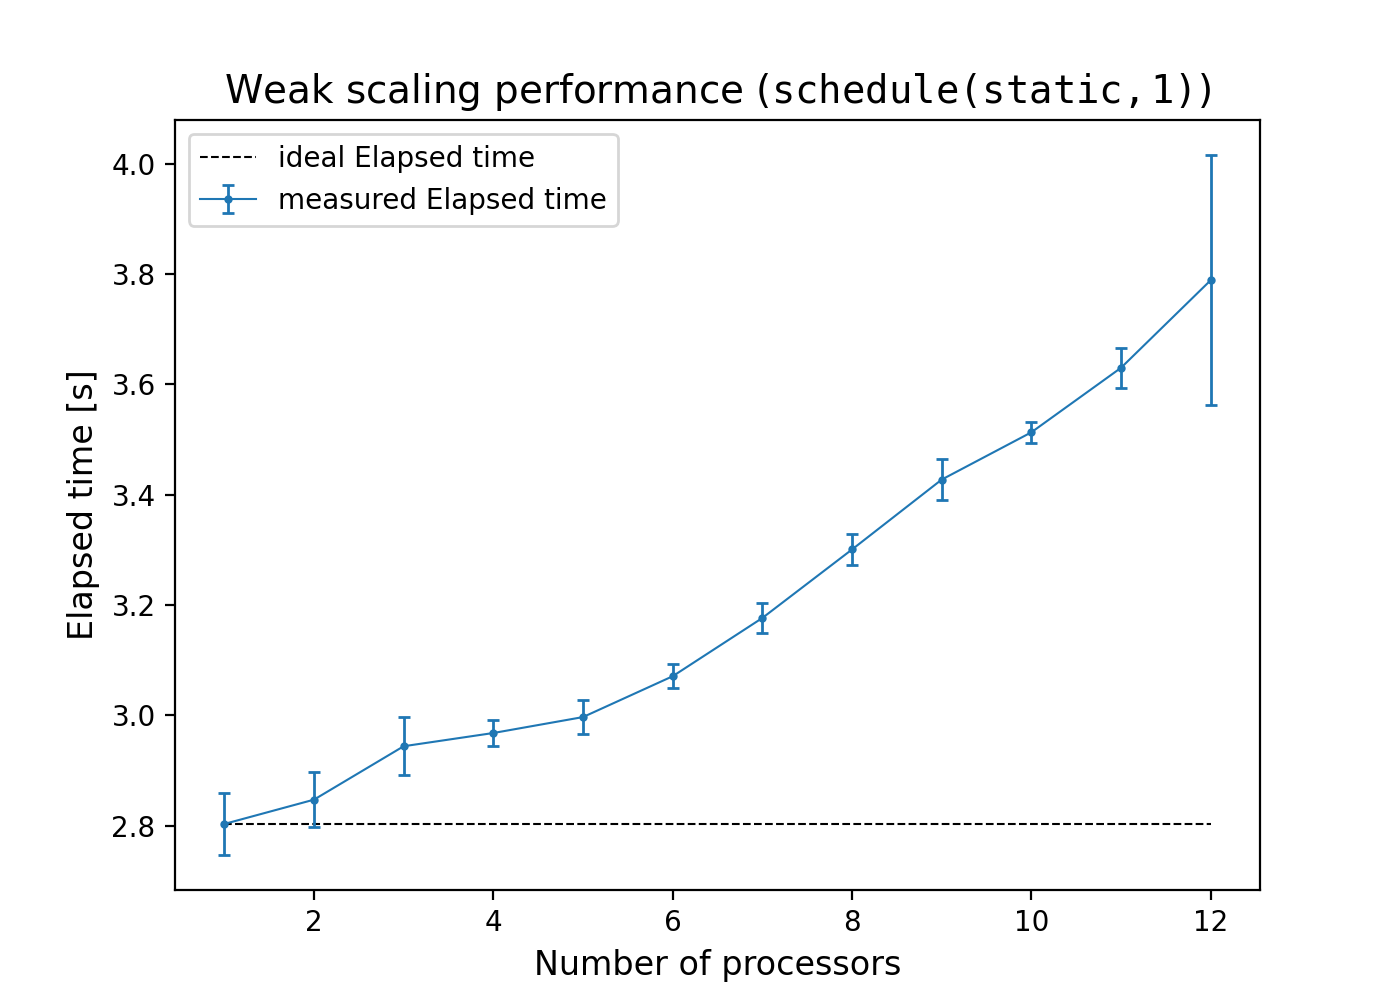
\includegraphics[width=0.42\textwidth]{threadsVStime_weak_collapse.png}
    \null\hfill
    \\
    \null\hfill
    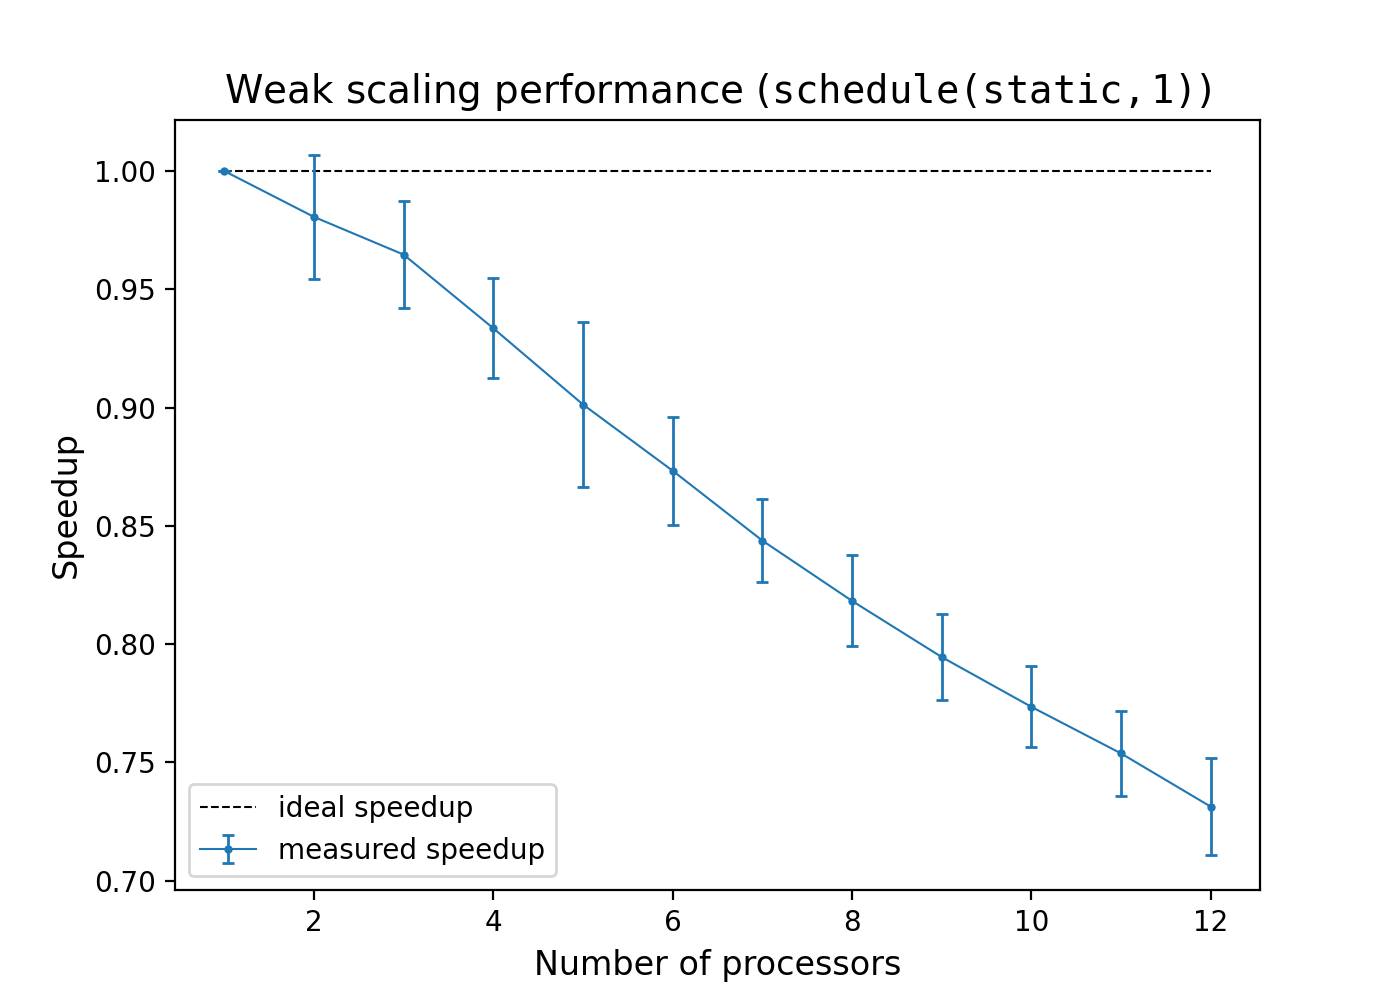
\includegraphics[width=0.42\textwidth]{threadsVSspeedup_weak.png}
    \null\hfill
    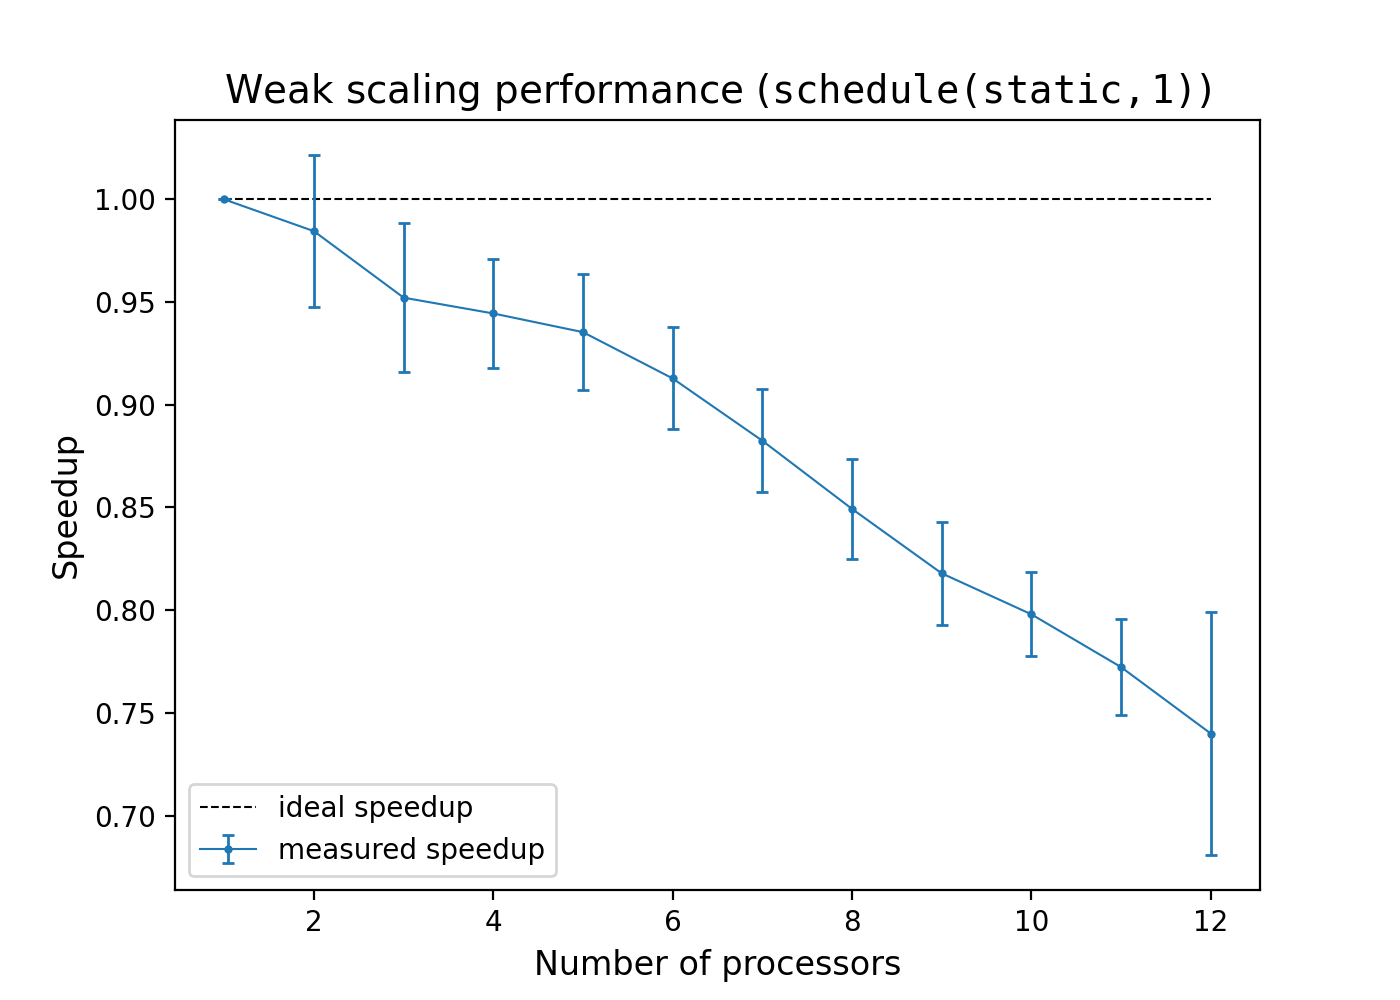
\includegraphics[width=0.42\textwidth]{threadsVSspeedup_weak_collapse.png}
    \null\hfill
    \caption{\label{fig:weak_scale}
    Performance plots (elapsed time and speedup) resulting from the \emph{weak scaling} conditions for a program with only the inner loop sped up (left column) and a program with the whole nested loop parallelized (right column). Both the programs are executed with the scheduling strategy fixed to \ompcode{schedule(static,1)}.}
\end{figure}

As highlighted by the plots in Figure~\ref{fig:weak_scale} representing the performance of the weak scaling conditions, the parallelization of both the Mandelbrot programs shows a behavior quite different from the ideal one. In fact, looking at the elapsed times on the first row, we can observe a \emph{linear} trend that deviates from the expected one by $T_P \sim T_1 + \varepsilon \cdot P$, with $\varepsilon \simeq 0.08~\rm{s}$ (empirically evaluated). The same phenomenon can be appreciated on the speedup plot (second row of Figure~\ref{fig:weak_scale}) where the negative trend can be described by $S_P \sim 1 - \varepsilon \cdot P/T_P$. Here, the $\varepsilon/T_P$ term can be read as the percentage drop in performance (with respect to the speedup) brought by each thread, that in this case amounts to about 2\%.

\begin{figure}[h!]
    \centering
    \null\hfill
    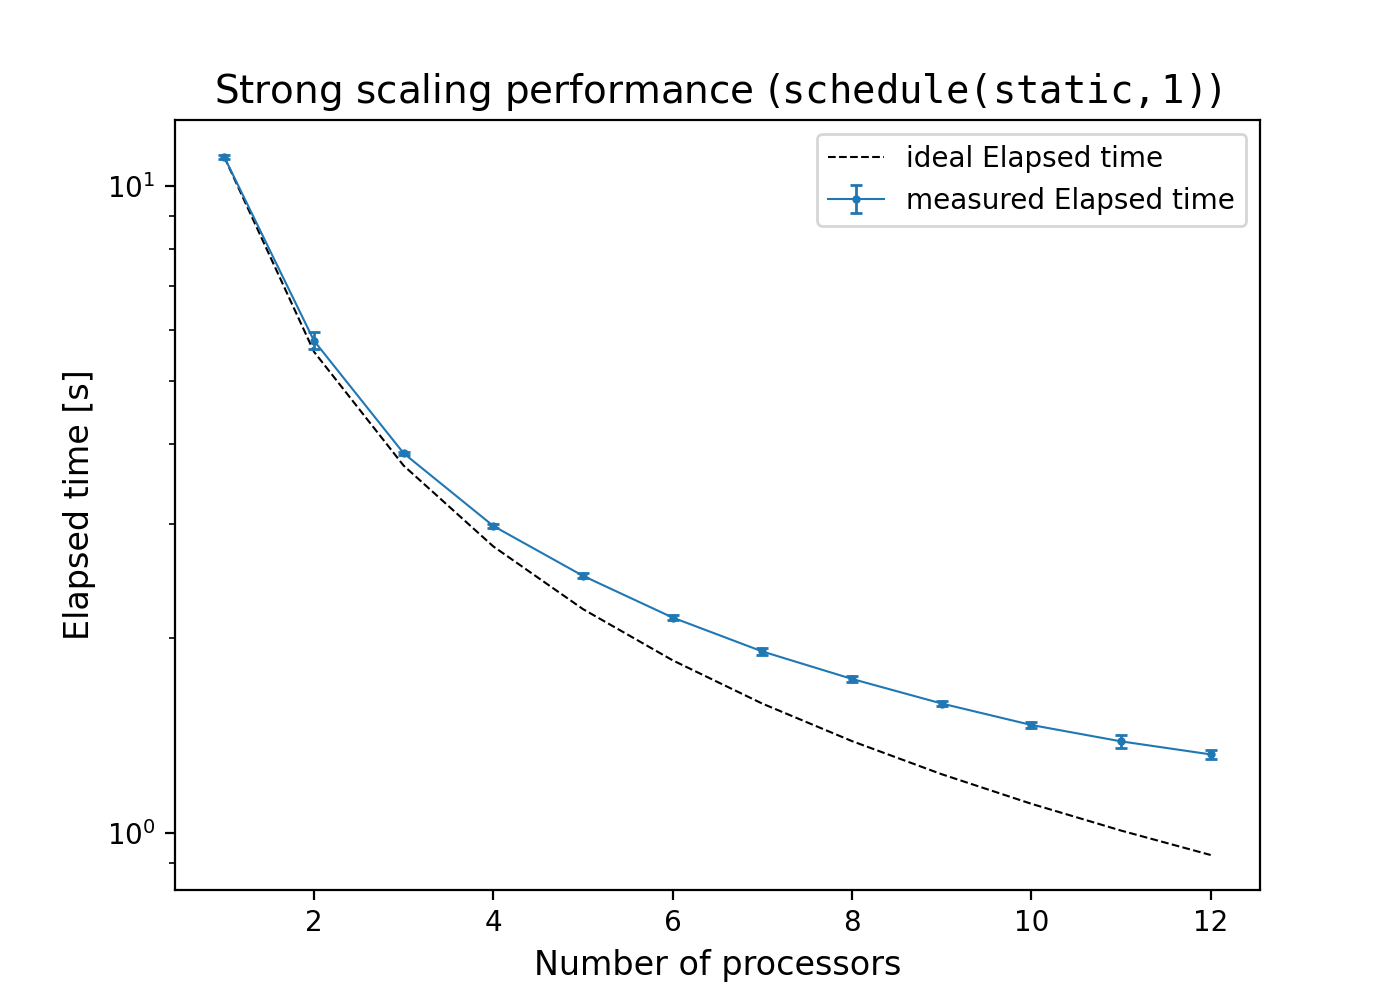
\includegraphics[width=0.42\textwidth]{threadsVStime_strong.png}
    \null\hfill
    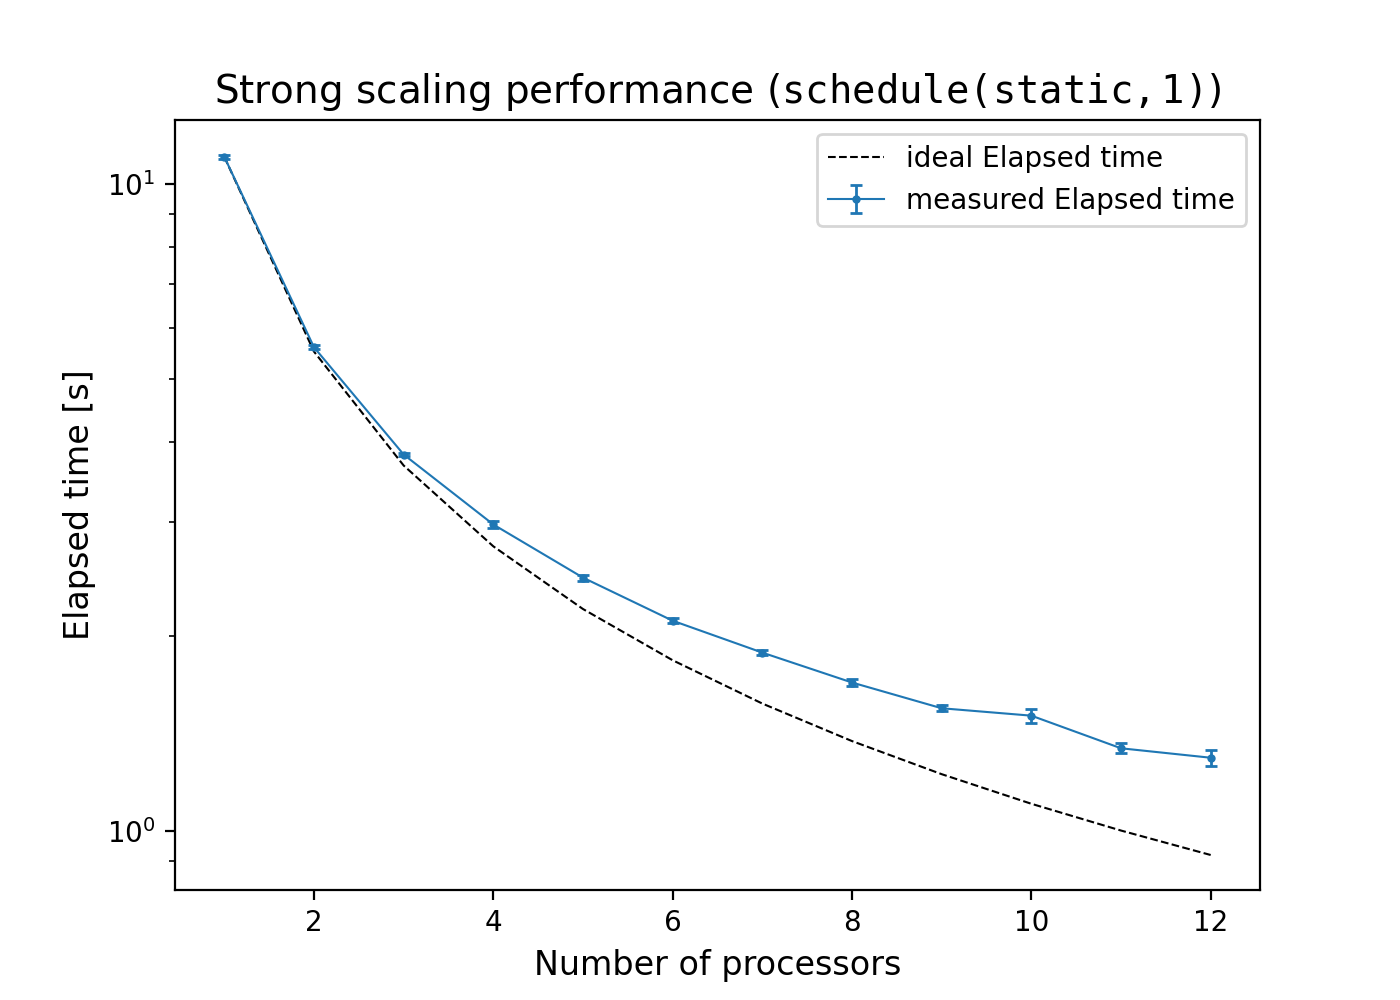
\includegraphics[width=0.42\textwidth]{threadsVStime_strong_collapse.png}
    \null\hfill
    \\
    \null\hfill
    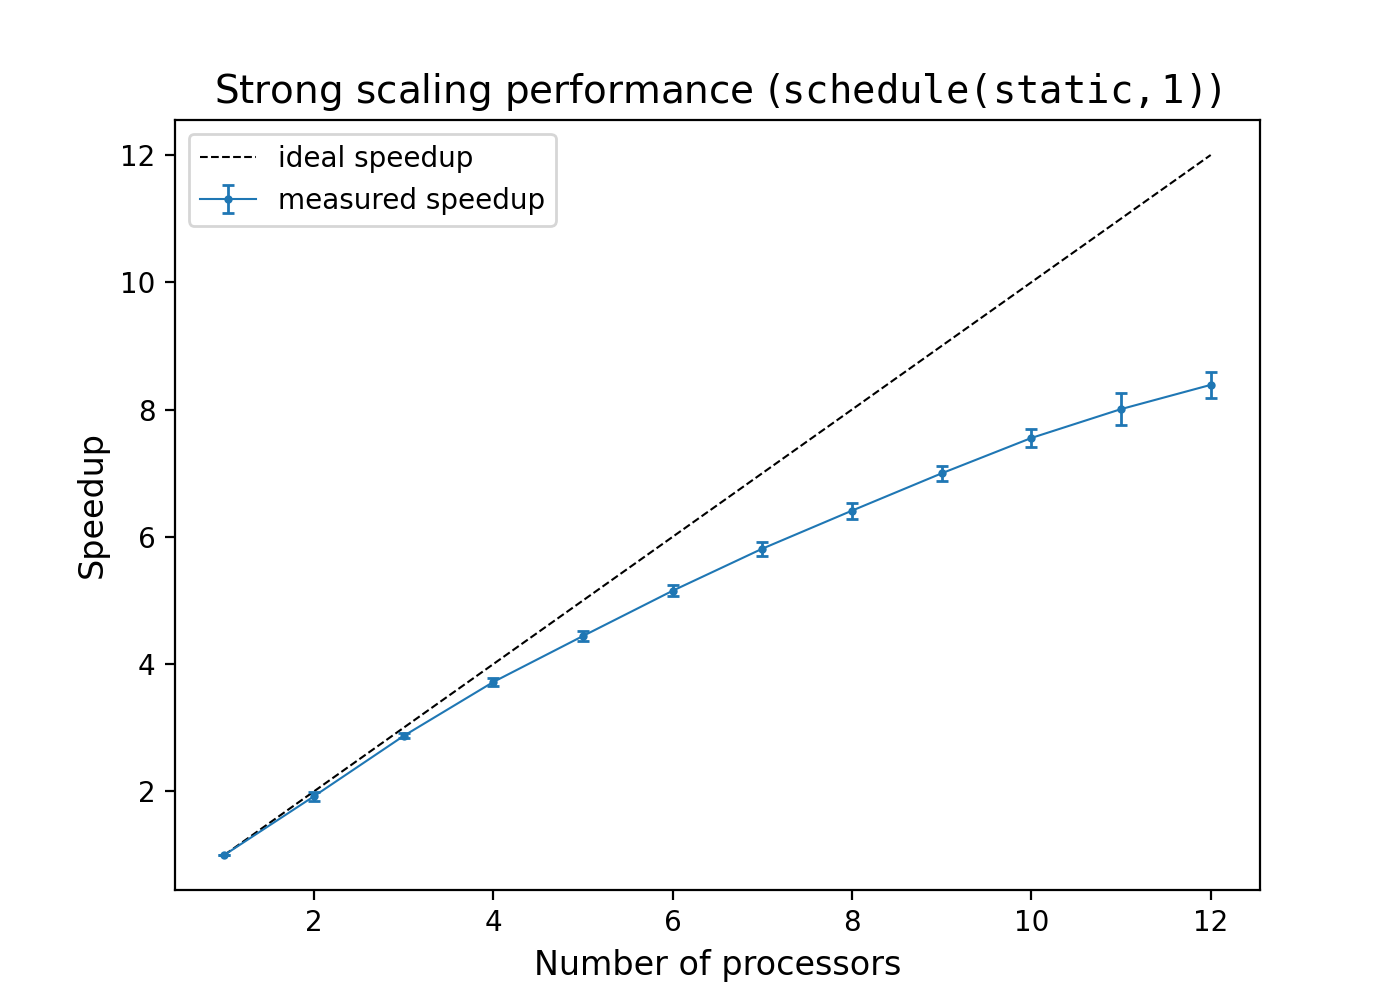
\includegraphics[width=0.42\textwidth]{threadsVSspeedup_strong.png}
    \null\hfill
    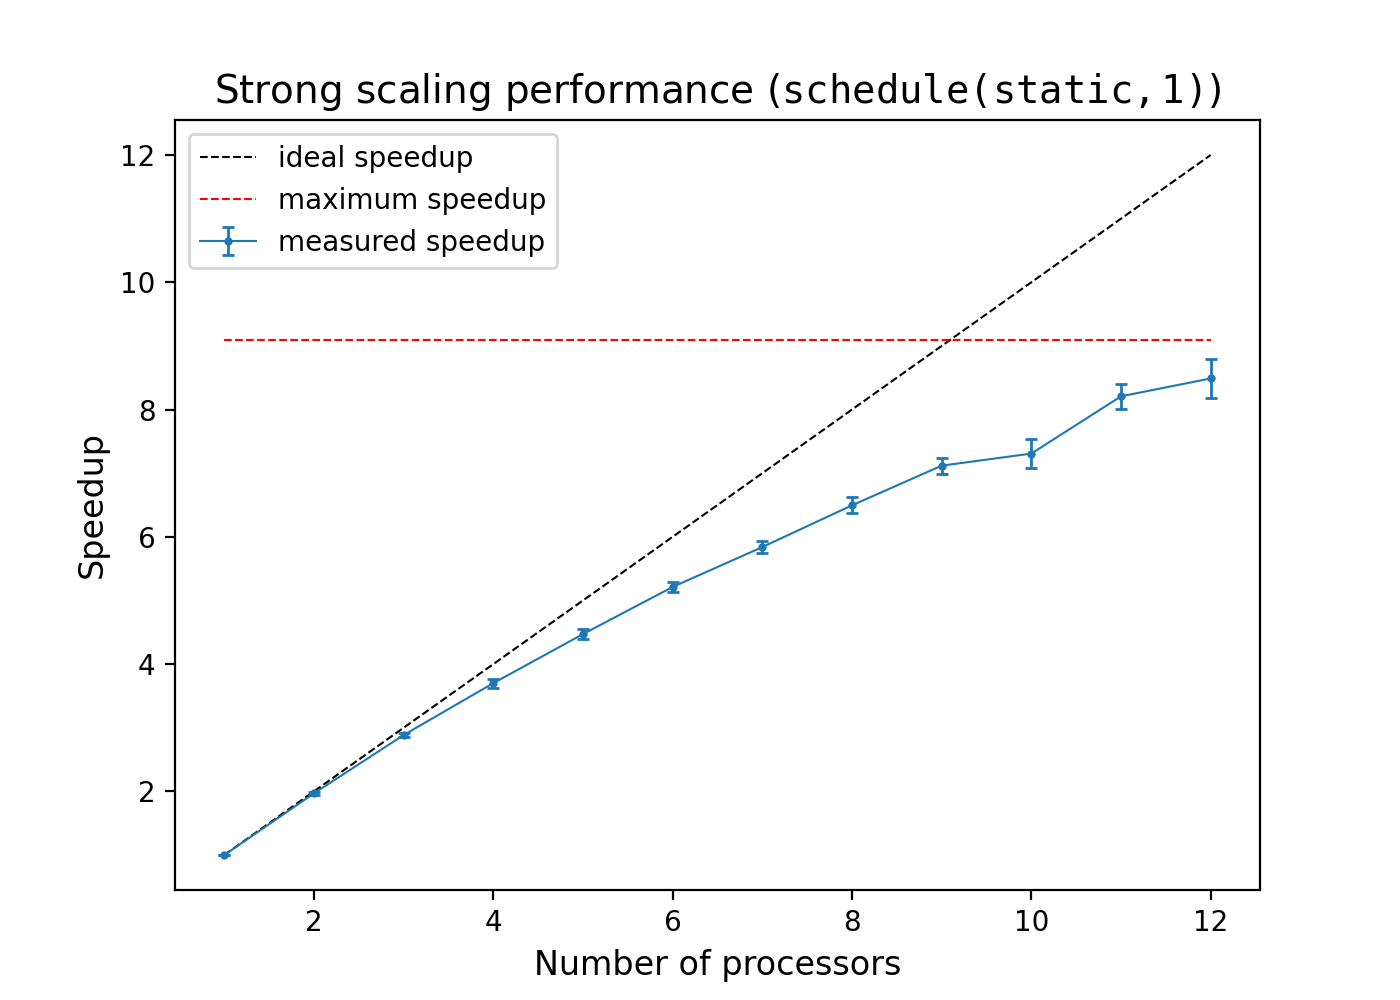
\includegraphics[width=0.42\textwidth]{threadsVSspeedup_strong_collapse.png}
    \null\hfill
    \caption{\label{fig:strong_scale}
    Performance plots (elapsed time and speedup) resulting from the \emph{strong scaling} conditions for a program with only the inner loop sped up (left column) and a program with the whole nested loop parallelized (right column). Both the programs are executed with the scheduling strategy fixed to \ompcode{schedule(static,1)}.}
\end{figure}

Also the plots reported in Figure~\ref{fig:strong_scale} representing the performance with the strong scaling conditions show a significant deviance from the ideal behavior, namely $T_P = T_1/P$ and $S_P = P$. The latter plots confirm what derived from the discussion of weak scaling, namely that the computing threads seem to perform slightly worse than expected, accumulating an overhead that becomes more and more significant with the increasing of the involved threads. This is clearly in accordance with the \emph{Work Law}. Moreover, relying on the \emph{Span Law}, the plots on the second row of Figure~\ref{fig:strong_scale} can be used to give an estimate, or better saying a lower bound of the parallelism intrinsic to the Mandelbrot program.
